\documentclass[11pt,a4paper%
addpoints, 
answers%
]{exam}
% \documentclass[a4paper,10pt]{exam}
\usepackage[applemac]{inputenc}
\usepackage[OT1,T1]{fontenc}
\usepackage{times}
\usepackage{setspace}
\usepackage{lscape}
\usepackage{amsmath,amssymb}
\usepackage{fancyvrb}
\usepackage{multirow}
\usepackage{float}
\usepackage{hyperref}
\usepackage{listings}
\usepackage{verbatim}
\usepackage{enumitem}
\usepackage{color}
\usepackage{graphicx}
\usepackage{rotating}
\usepackage{subcaption}
\usepackage{textcomp}
\usepackage{caption}
\usepackage{pdfpages}


\definecolor{mygreen}{rgb}{0,0.6,0}
\definecolor{mygray}{rgb}{0.5,0.5,0.5}
\definecolor{mymauve}{rgb}{0.58,0,0.82}

\setlength{\textwidth}{160mm}
\setlength{\textheight}{230mm}
%\setlength{\oddsidemargin}{-5mm}
\setlength{\topmargin}{-10mm}

\newcommand{\ns}{\!\!\!}
\newcommand{\e}{\varepsilon}
\newcommand{\be}{\beta}
\newcommand{\s}{\sigma}
\newcommand{\vv}{\vspace{.5cm}}
\newcommand{\beps}{\boldsymbol{\epsilon}}
\newcommand{\sumin}{\sum_{i=1}^n}
\newcommand{\bg}[1]{\mbox{\boldmath{$#1$}}}
\DeclareMathOperator{\plim}{plim}
\DefineVerbatimEnvironment{code}{Verbatim}{fontsize=\small}
\DefineVerbatimEnvironment{example}{Verbatim}{fontsize=\small}

\def\by{\mathbf{y}}
\def\bx{\mathbf{x}}
\def\ba{\mathbf{a}}
\def\bb{\mathbf{b}}
\def\be{\mathbf{e}}
\def\bu{\mathbf{u}}
\def\bv{\mathbf{v}}
\def\bz{\mathbf{z}}

%===========
%Greek letter vectors
%===========
\def\bbeta{\mbox{\boldmath $\beta$}}
\def\bgamma{\mbox{\boldmath $\gamma$}}
\def\bvareps{\mbox{\boldmath $\varepsilon$}}
\def\bleta{\mbox{\boldmath $\eta$}}
\def\bmu{\mbox{\boldmath $\mu$}}
\def\btheta{\mbox{\boldmath $\theta$}}
\def\bsigma{\mbox{\boldmath $\sigma$}}
\def\blambgam{\mbox{\boldmath $\lambda_{\gamma}$}}
\def\blambbet{\mbox{\boldmath $\lambda_{\beta}$}}
\def\blambda{\mbox{\boldmath $\lambda$}}

%===========
%Matrices
%===========
\def\bX{\mathbf{X}}
\def\bD{\mathbf{D}(\bsigma)}
\def\bV{\mathbf{V}(\bsigma)}
\def\bVinv{\mathbf{V}^{-1}(\bsigma)}
\def\bR{\mathbf{R}(\bsigma)}
\def\bA{\mathbf{A}}
\def\bB{\mathbf{B}}
\def\bZ{\mathbf{Z}}
\def\bIn{\mathbf{I_{N}}}
\def\bIm{\mathbf{I_{m}}}
\def\bIni{\mathbf{I_{n}}}
\def\SSW{\mathrm{SSW}}
\def\SSB{\mathrm{SSB}}
\def\Normal{\mathcal{N}\!}

%===========
%Parentheses, etc.
%===========
\def\op{\left(}
\def\cp{\right)}
\def\oc{\left[}
\def\cc{\right]}
\def\ok{\left\{}
\def\ck{\right\}}

%===========
%Statistical functions and real numbers.
%===========
\def\exE{\mathbb{E}}
\def\Real{\mathbb{R}}
\def\Var{\mathbb{V}ar}
\def\Proba{\mathbb{P}}

%===========
%Listings and hyperlink settings
%===========
\hypersetup{colorlinks=true,linkcolor=blue,citecolor=blue, urlcolor=blue}
\urlstyle{tt}
%\lstset{language=R, basicstyle=\footnotesize\ttfamily,}
\definecolor{lightgray}{gray}{0.95}

\lstset{ %
%  language=R, 
  basicstyle=\scriptsize\ttfamily,
  backgroundcolor=\color{lightgray},   % choose the background color; you must add \usepackage{color} or \usepackage{xcolor}
%  breakatwhitespace=false,         % sets if automatic breaks should only happen at whitespace
%  breaklines=true,                 % sets automatic line breaking
%  captionpos=b,                    % sets the caption-position to bottom
%  commentstyle=\color{mygreen},    % comment style
%  deletekeywords={...},            % if you want to delete keywords from the given language
%  escapeinside={\%*}{*)},          % if you want to add LaTeX within your code
%  extendedchars=true,              % lets you use non-ASCII characters; for 8-bits encodings only, does not work with UTF-8
  frame=single,                    % adds a frame around the code
%  keepspaces=true,                 % keeps spaces in text, useful for keeping indentation of code (possibly needs columns=flexible)
%  keywordstyle=\color{blue},       % keyword style
%  language=Octave,                 % the language of the code
%  morekeywords={*,...},            % if you want to add more keywords to the set
  numbers=left,                    % where to put the line-numbers; possible values are (none, left, right)
  numbersep=5pt,                   % how far the line-numbers are from the code
  numberstyle=\tiny\color{mygray}, % the style that is used for the line-numbers
%  rulecolor=\color{black},         % if not set, the frame-color may be changed on line-breaks within not-black text (e.g. comments (green here))
  showspaces=false,                % show spaces everywhere adding particular underscores; it overrides 'showstringspaces'
%  showstringspaces=false,          % underline spaces within strings only
%  showtabs=false,                  % show tabs within strings adding particular underscores
%  stepnumber=2,                    % the step between two line-numbers. If it's 1, each line will be numbered
%  stringstyle=\color{mymauve},     % string literal style
%  tabsize=2,                       % sets default tabsize to 2 spaces
%  title=\lstname                   % show the filename of files included with \lstinputlisting; also try caption instead of title
}

%===========
%Special Environments
%===========
\newenvironment{exercices}{\newcounter{moncompteur}\begin{list}
   {\bfseries Ex. \arabic{moncompteur}}{\usecounter{moncompteur}
     \setlength{\labelwidth}{2.6em}\setlength{\leftmargin}{3.1em}}}{\end{list}}
%\renewcommand{\labelenumi}{\bfseries\alph{enumi})}
\newcommand{\splus}[3][0]{\texttt{>~#2}\ \ \ \ \textit{#3}\\[#1mm]}

\newenvironment{exo}
{\begin{center}\setlength{\textwidth}{140mm} \underline{Exercise:} \begin{minipage}[t]{120mm}}
{\end{minipage}\setlength{\textwidth}{160mm}\end{center}}


\footer{}{Page \thepage\ of \numpages}{}

\begin{document}

\noindent \textsc{University of Geneva} \hfill S411001 GLAM\\
Prof. Eva Cantoni \hfill Spring 2022\\
\noindent
\makebox[\linewidth]{\rule{\textwidth}{0.4pt}}\\[1.5ex]
\hfill \textbf{Exam} \hfill \normalfont{June 10th, 2022}\\
\makebox[\linewidth]{\rule{\textwidth}{0.4pt}}\\

\bigskip

\setlength{\parskip}{1ex plus 0.5ex minus 0.2ex}
\parindent=0cm
\linespread{1.1}


{\Large \textbf{Exercise 1} \hfill (42 points)}

\bigskip 

The dataset \texttt{CO2} gives the result of a controlled experiment conducted on $12$ individual plants. 
	Each of these plants was successively exposed to 7 different CO2 concentrations while their CO2 uptake rates were measured. 
	Some of the plants were exposed to a cold treatment, others were not. 
	Each of the plants, of the species \textit{Echinochloa crus-galli}, has one of two origins: Quebec or Mississipi. 
	The goal of the experiment is to determine if the cold treatment has an impact on the growth of plants, for which the absorption of CO2 is a proxy.
	
	The dataset contains 84 observations with 5 columns: 
	\begin{itemize}
		\item \texttt{Plant}: a factor  identifying each plant.
		\item \texttt{Type}: a factor with levels \texttt{Quebec} or \texttt{Mississippi} indicating the origin of the plant.
		\item \texttt{Treatment}: a factor with levels \texttt{nonchilled} or \texttt{chilled}, indicating if a plant was exposed to a cold treatment or not. 
		\item \texttt{conc}: a numeric vector giving the CO2 concentration to which the plants were exposed.
		\item \texttt{uptake}: a numeric vector giving the CO2 uptake rates.		
	\end{itemize}
	
We start by naively fitting two GLM models to this data as presented in Output~\ref{out.glm1} and Output~\ref{out.glm2}.

\begin{center}
\begin{verbatim}
> fit_1 <- glm(uptake ~ conc + Treatment + Type, family = gaussian(),data=CO2)
> fit_1

Call:  glm(formula = uptake ~ conc + Treatment + Type, family = gaussian(), 
    data = CO2)

Coefficients:
     (Intercept)              conc  Treatmentchilled   TypeMississippi  
        29.25981           0.01773          -6.85952         -12.65952  

Degrees of Freedom: 83 Total (i.e. Null);  80 Residual
Null Deviance:	    9707 
Residual Deviance: 3068 	AIC: .....

> logLik(fit_1)
'log Lik.' -270.3099 (df=.....)

> sigma(fit_1)
[1] 6.193074

\end{verbatim}
\end{center}


\begin{center}
\begin{verbatim}

> fit_2 <- glm(log(uptake) ~ log(conc-92) + Treatment + Type, family = gaussian(),data=CO2)
> fit_2

Call:  glm(formula = log(uptake) ~ log(conc - 92) + Treatment + Type, 
    family = gaussian(), data = CO2)

Coefficients:
     (Intercept)    log(conc - 92)  Treatmentchilled   TypeMississippi  
          2.7085            0.1774           -0.2993           -0.4896  

Degrees of Freedom: 83 Total (i.e. Null);  80 Residual
Null Deviance:	    17.69 
Residual Deviance: 2.459 	AIC: -48.22

> sigma(fit_2)
[1] 0.1753334

\end{verbatim} 
\end{center}

\begin{questions}
\question[1] Model 1 and Model 2 have been fitted using the function \texttt{glm}. Which other \texttt{R} function could have been used instead for this case?

\begin{solution}
Function  \texttt{lm}, because Gaussian family.
\end{solution}

\question[2] \label{mod1vsmod2} Based on the diagnostic plots of Figure~\ref{fig:fig_1}, which of Model 1 or Model 2 seems to be the more relevant? 
\begin{solution}
	GLM Model 2 seems better: its residuals are closer to normality than the residuals of GLM Model 1, and the trend in the "residuals vs fitted values" plot is less pronounced.
\end{solution}

\begin{figure}[htbp!]
\caption{Diagnostic plots of the fits of the Model 1 (two left hand side panels) and Model 2 (two right hand side panels)}
\begin{center}
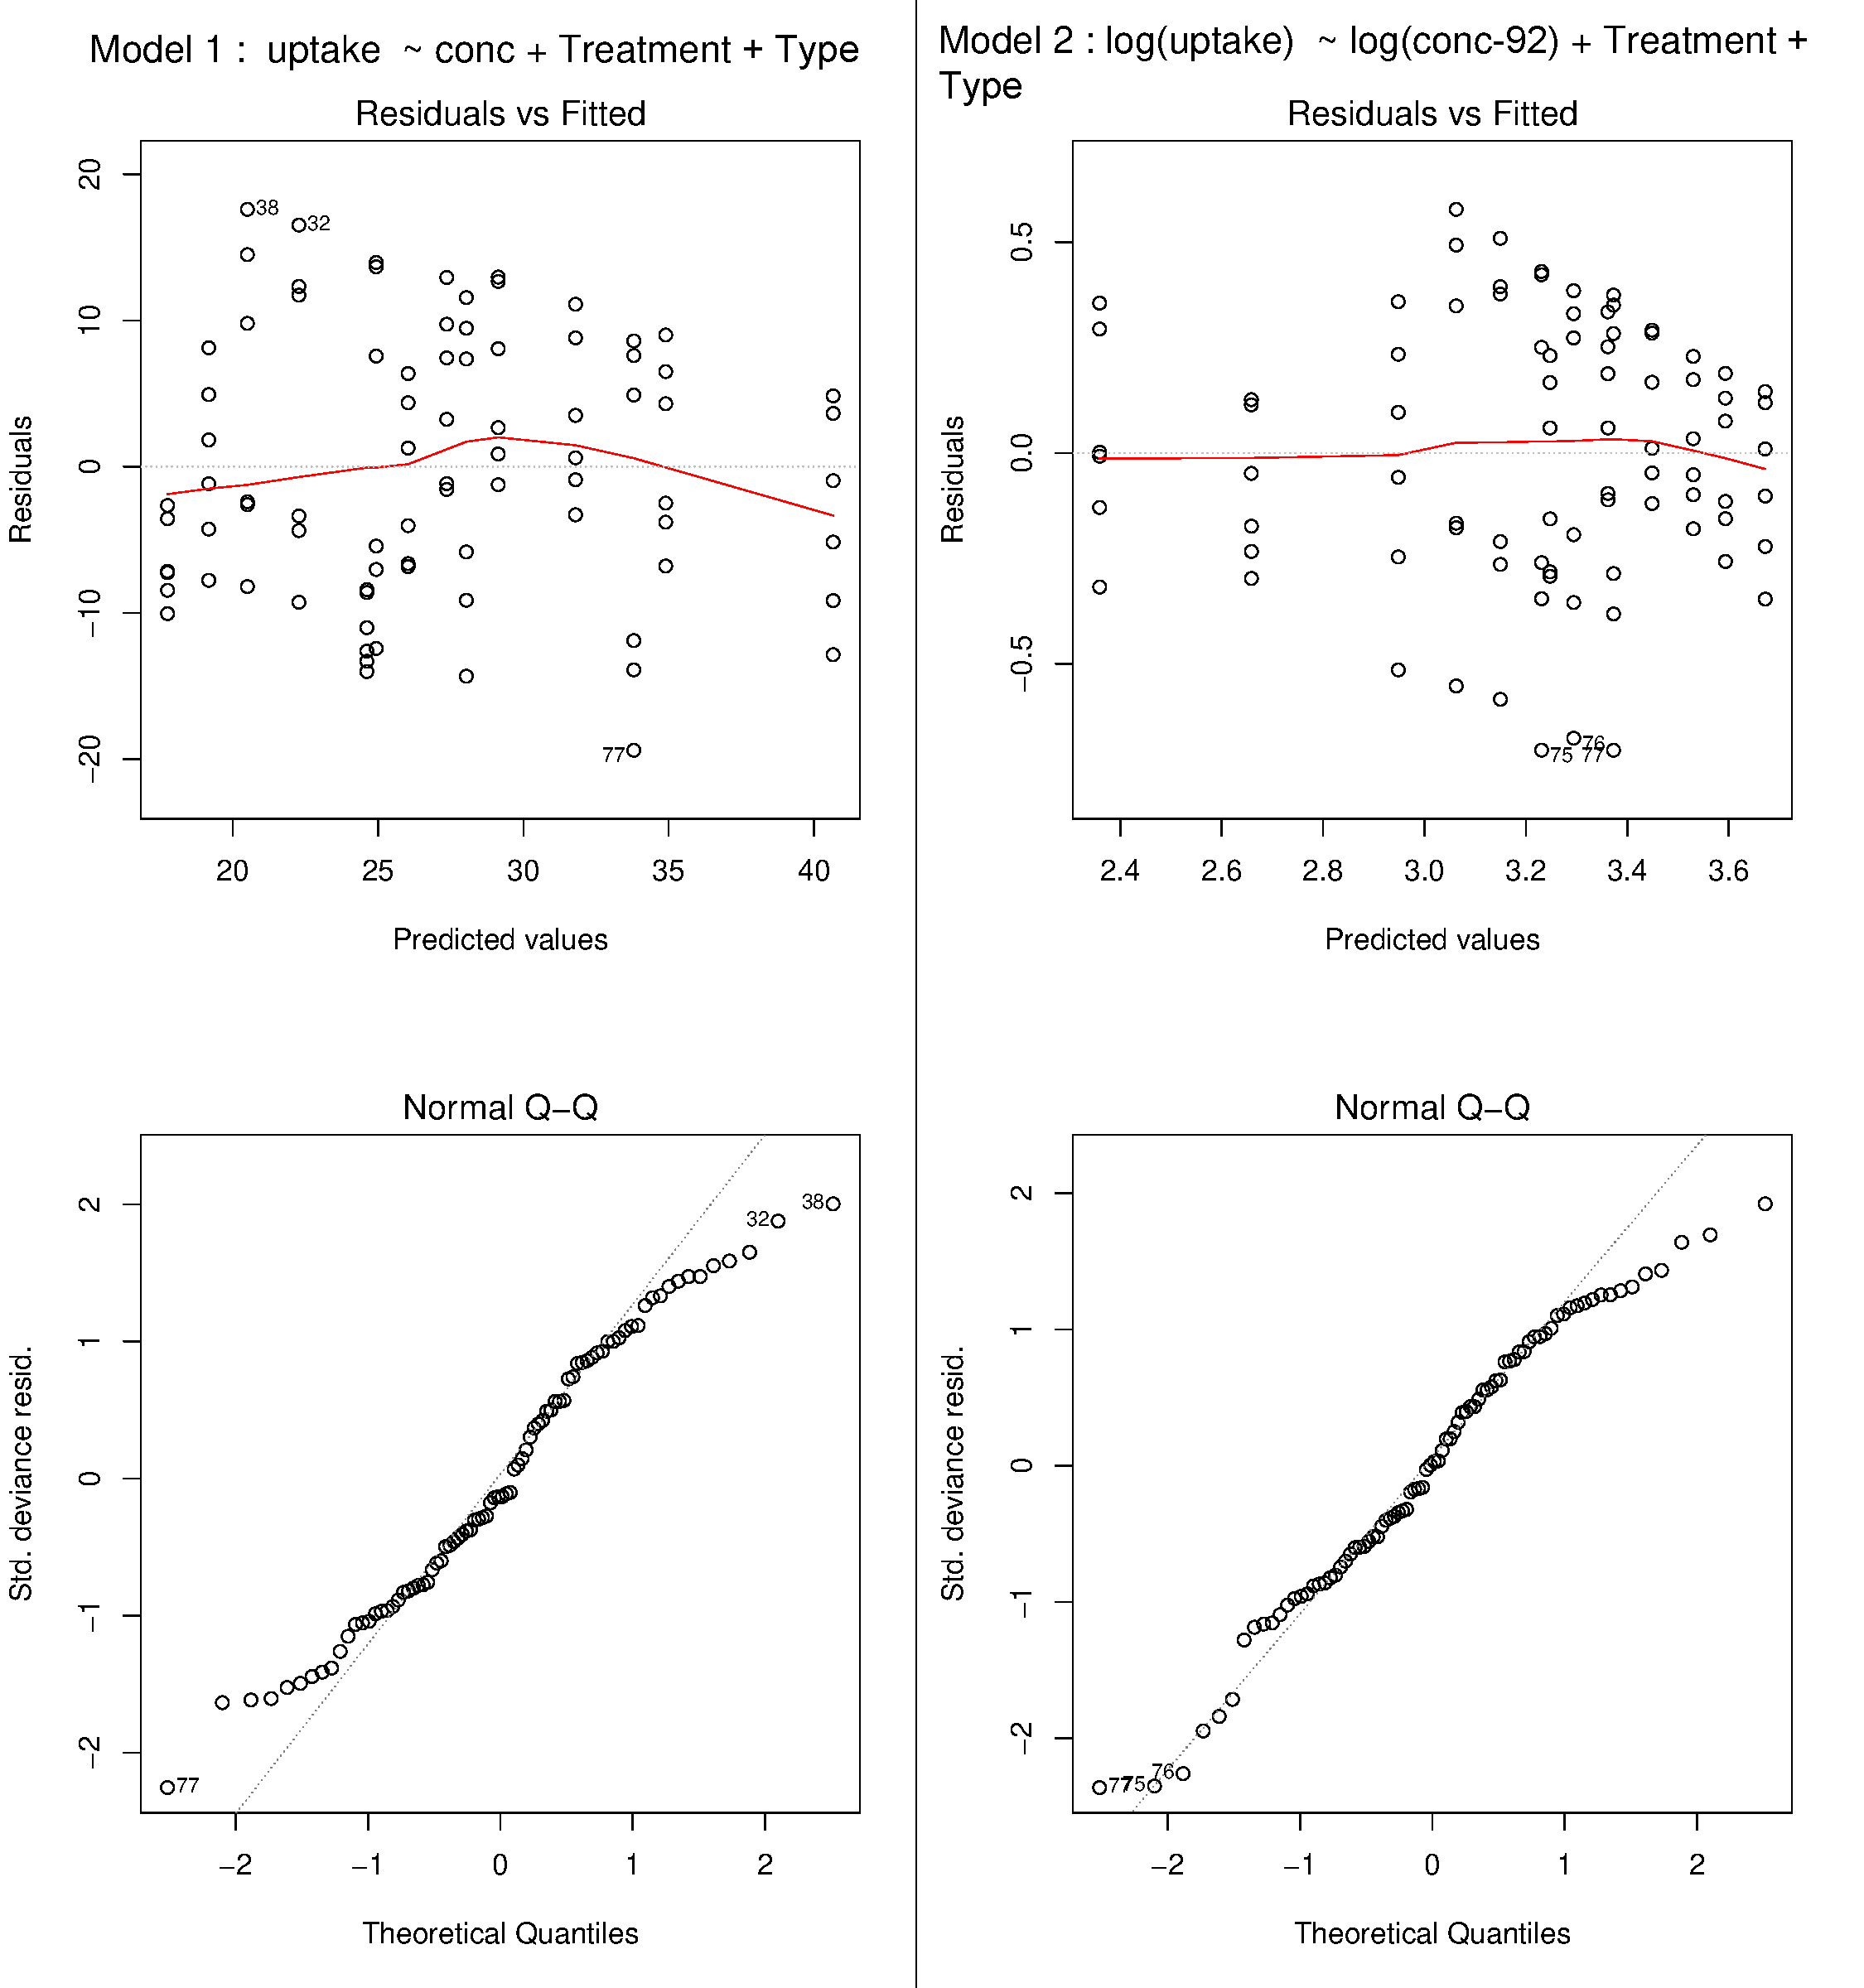
\includegraphics[height = 4.2in]{fig1_exa.pdf}
\label{fig:fig_1}
\end{center}
\end{figure}

\newpage
\question[3] For Model 1 and Model 2 give the value of the deviance $D$ and of the scaled deviance $D^*$. Perform a goodness-of-fit test at $5\%$ level to test whether the model is good.

\begin{solution}
For Model 1, from Output~\ref{out.glm1}, $D=3068$ and $\hat{\phi} = \hat{\sigma}^2 = 6.19^2$, therefore $D^* = 3068/6.19^2 = 80.07$.

For Model 2, from Output~\ref{out.glm2}, $D=2.459$ and $\hat{\phi} = \hat{\sigma}^2 = 0.175^2$, therefore $D^* = 2.459/0.175^2 = 80.29$.

The $95\%$ quantile of a $\chi^2_{79}$ distribution is $100.75$ (and the $95\%$ quantile of a $\chi^2_{80}$ distribution is $101.88$), therefore the null hypothesis $H_0$: ``the model is good''  is not rejected nor for Model neither for Model 2.

\end{solution}

\question[2] Compute the Akaike Information Criterion (AIC) of Model 1.
\begin{solution}

AIC = -2 loglik + 2* (nb of parameters) = $-2 * (-270.3099) + 2*5 = 550.6198$.

We also accept the solution AIC = $-2 * (-270.3099) + 2*4 = 548.6198$

\end{solution}


\question[2]  Why can't you naively compare the AIC of Model 1 and 2 ? Explain briefly, without doing it, how you could compute the AIC of the second model in order to compare the two models.
	\begin{solution}
		We can't naively compare the AIC of Model 1 and 2 because the models don't have the same \textit{response}. 
		
		The second model actually models $\log(uptake)$ rather than uptake, i.e. it assumes that \texttt{uptake} follows a log-normal distribution. 
		AIC of Model 2 can be computed by hand. Number of parameters is $k = 4 + 1$ and the likelihood can be computed as \\
		$$l = \sum_i \log\left(\frac{1}{\texttt{uptake}_i \, \hat{\sigma}} \varphi\left(\frac{\log(\texttt{uptake}_i) - \hat{y}_i} {\hat{\sigma}}\right)\right) \, .$$  
		where $\varphi$ is the density of a standard normal, using the fact that the density of a standard log-normal random variable is $\frac{1}{x}\varphi(x)$. 
			The AIC is then $2( k - l)$.
	\end{solution}
\question[2]
 Figure~\ref{fig:fig_2} shows, for Model 2, the residuals as a function of the randomized residuals. Explain what you observe and why.
 \begin{solution}
Randomized residuals and residuals are proportional. This is expected since we are using a gaussian family. Randomized residuals are thus $\Phi(F(y_i; \hat{\mu}_i, \hat{\sigma})) = \Phi^{-1}(\Phi((y_i - \hat{y}_i) / \hat{\sigma})) = r / \hat{\sigma}$ where $r$ are the model's residuals. 
\end{solution}
	\begin{figure}[htbp]
		\centering
		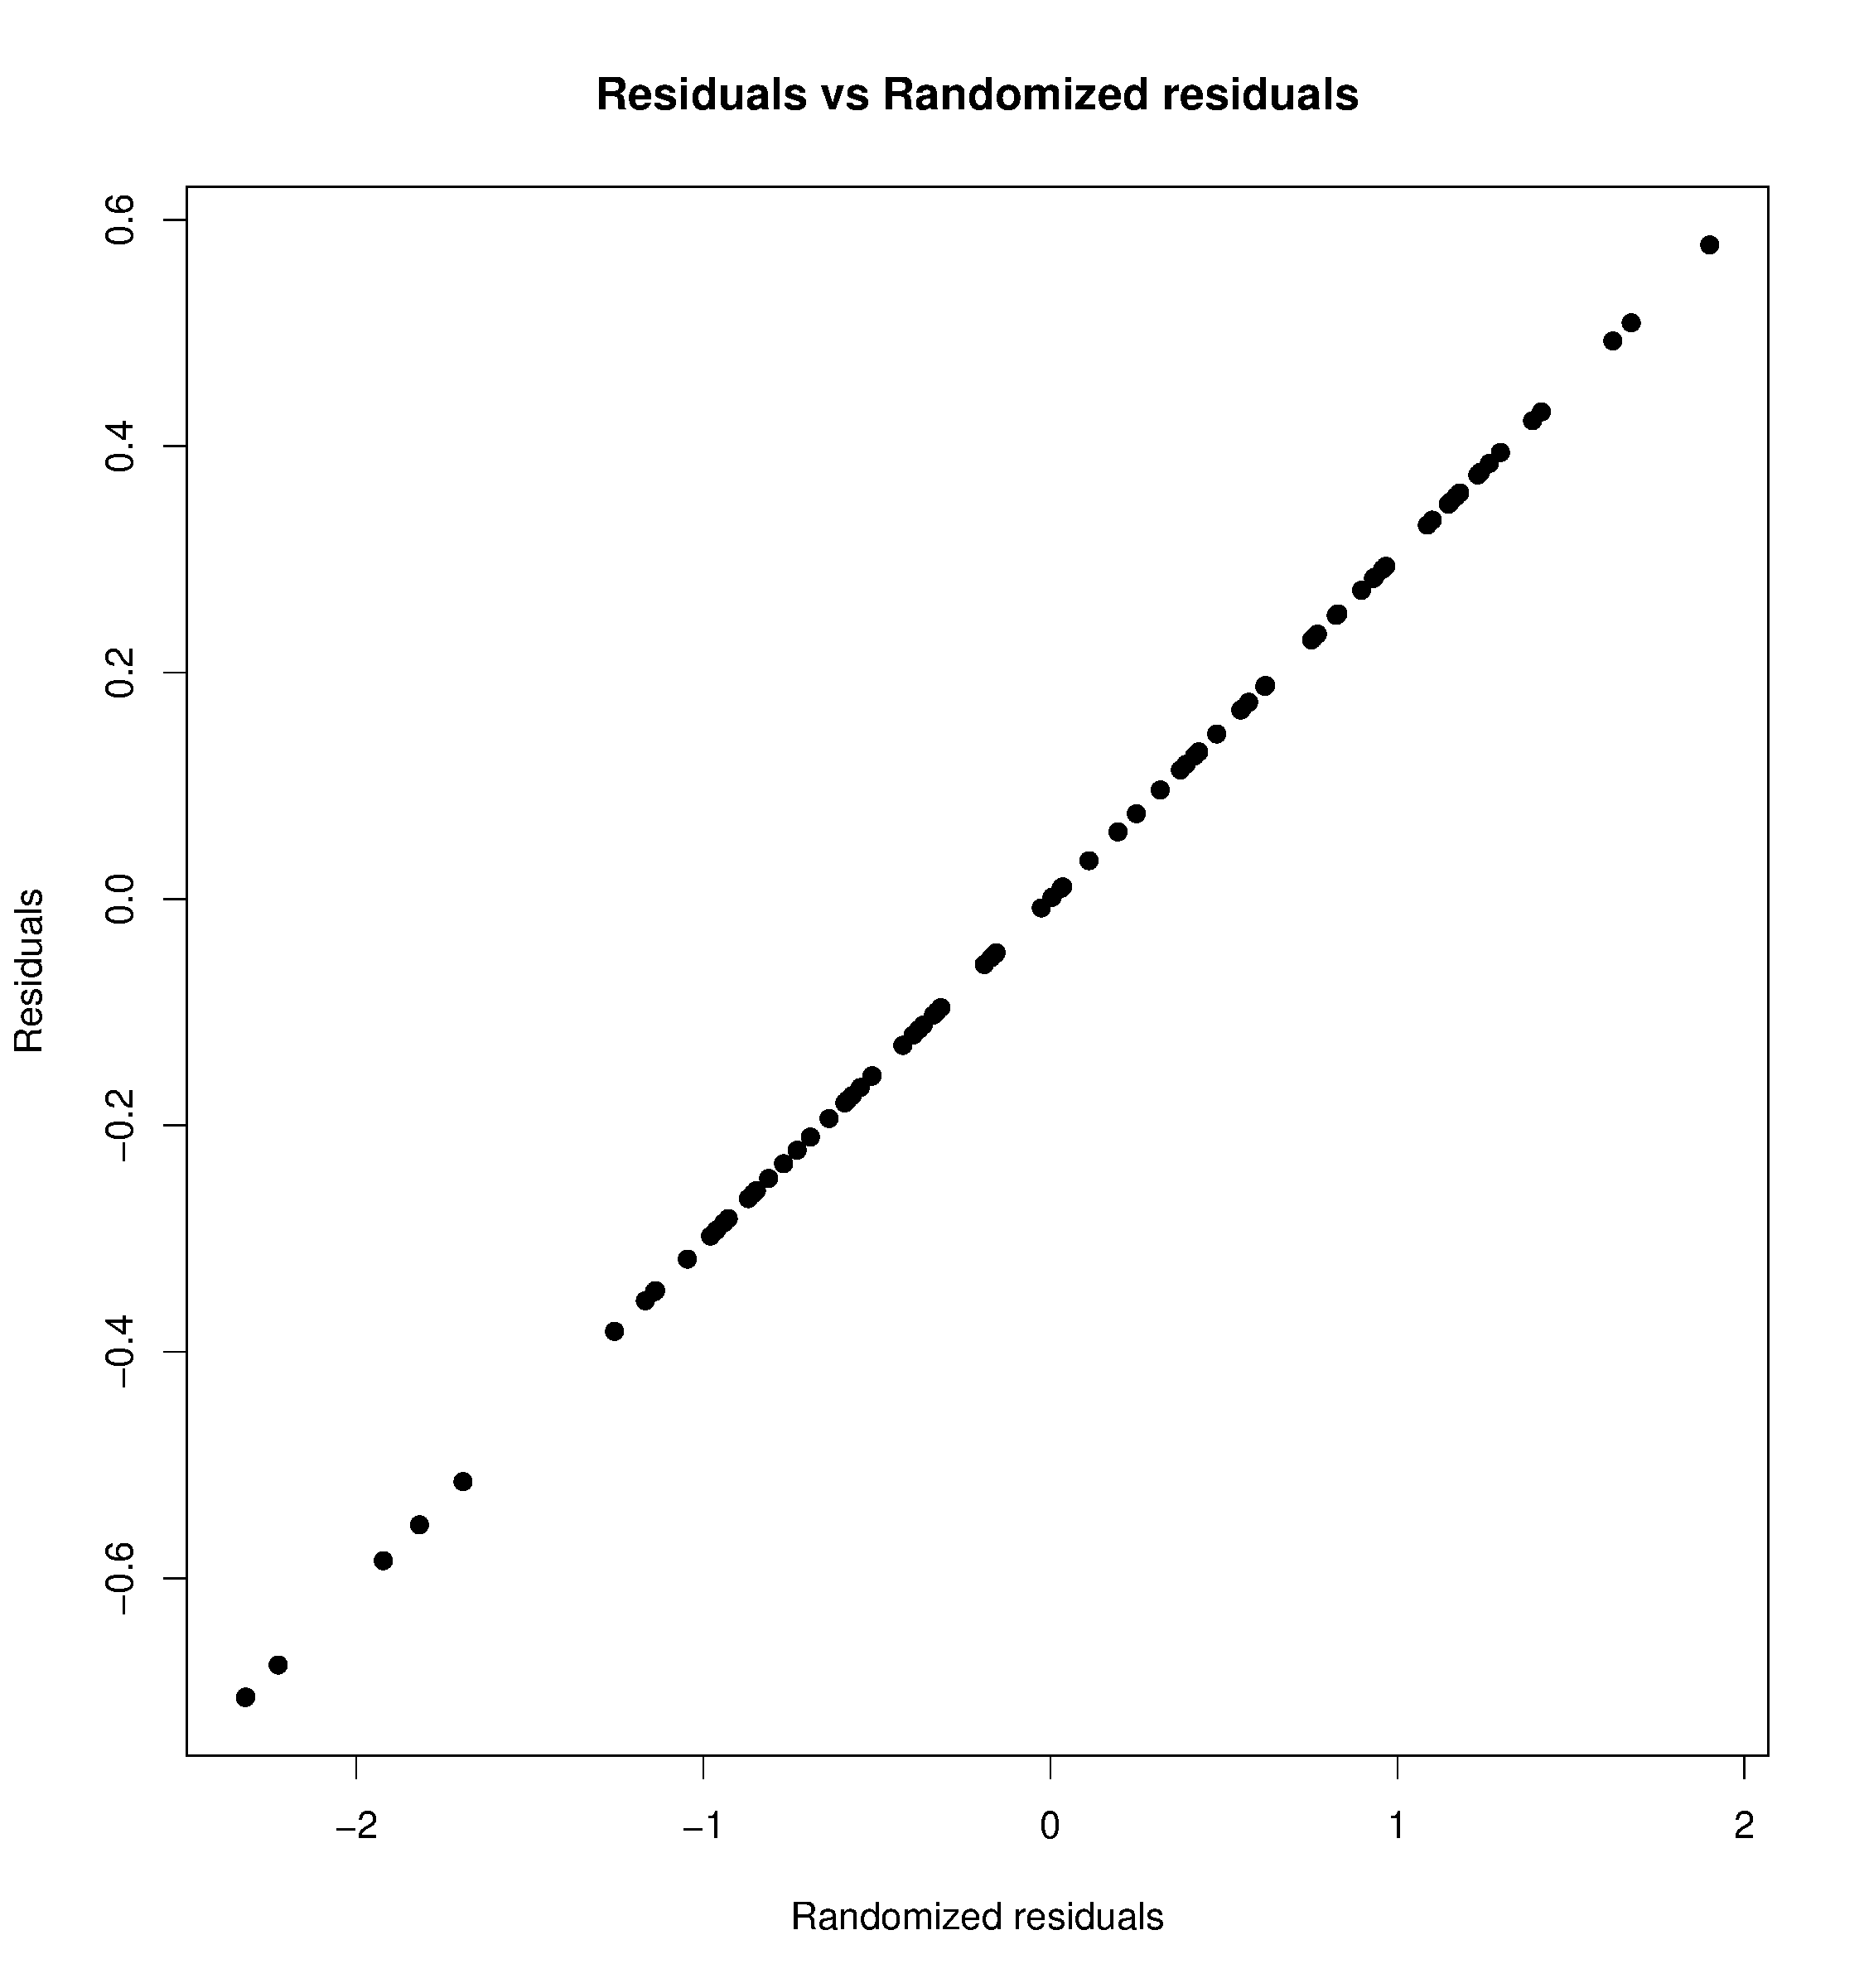
\includegraphics[height = 4.5in]{fig3_exa.pdf}
		\caption{Residuals vs randomized residuals of Model 2.}
		\label{fig:fig_2}
	\end{figure} 


\newpage
\question[2] We fitted a third GLM model, Model 3 in Output~\ref{out.glm3}. What is wrong with Model 3? Why are some coefficients estimated as `NA'?
\begin{solution}
The variable Plant is nested in the variables Treatment and Type, hence the model is non-identifiable. This is why the coefficients for Type and Treatment are \texttt{NA} .	
\end{solution}

\begin{center}
\begin{verbatim}
> fit_3 <- glm(log(uptake) ~ log(conc-92) + Plant + Treatment + Type , family = gaussian(),
  data=CO2)
> summary(fit_3)

Call:
glm(formula = log(uptake) ~ log(conc - 92) + Plant + Treatment + 
    Type, family = gaussian(), data = CO2)

Deviance Residuals: 
     Min        1Q    Median        3Q       Max  
-0.46623  -0.06363  -0.00039   0.06051   0.26150  

Coefficients: (2 not defined because of singularities)
                  Estimate Std. Error t value Pr(>|t|)    
(Intercept)       2.314026   0.039827  58.101  < 2e-16 ***
log(conc - 92)    0.177382   0.007446  23.823  < 2e-16 ***
Plant.1          -0.911548   0.045756 -19.922  < 2e-16 ***
Plant.2          -0.199034   0.045756  -4.350 4.47e-05 ***
Plant.3           0.192827   0.045756   4.214 7.26e-05 ***
Plant.4           0.177825   0.045756   3.886 0.000226 ***
Plant.5           0.192450   0.045756   4.206 7.47e-05 ***
Plant.6           0.002603   0.045756   0.057 0.954785    
Plant.7          -0.168129   0.045756  -3.674 0.000459 ***
Plant.8          -0.232960   0.045756  -5.091 2.80e-06 ***
Plant.9          -0.359907   0.045756  -7.866 2.96e-11 ***
Plant.10         -0.019746   0.045756  -0.432 0.667381    
Plant.11          0.040542   0.045756   0.886 0.378577    
Treatmentchilled        NA         NA      NA       NA    
TypeMississippi         NA         NA      NA       NA    
---
Signif. codes:  0 ‘***’ 0.001 ‘**’ 0.01 ‘*’ 0.05 ‘.’ 0.1 ‘ ’ 1

(Dispersion parameter for gaussian family taken to be 0.0146551)

    Null deviance: 17.6913  on 83  degrees of freedom
Residual deviance:  1.0405  on 71  degrees of freedom
AIC: -102.47

Number of Fisher Scoring iterations: 2

\end{verbatim}
\end{center}


\question[2] We could fit an alternative model as in Output~\ref{out.glm4}.

\begin{center}
\begin{verbatim}
 fit_4 <- glm(uptake ~ log(conc-92) + Treatment + Type, family = gaussian(link="log"), 
 data=CO2)
\end{verbatim}
\end{center}

Is Model 4 the same as Model 2? Explain in details.

\begin{solution}
The two models are not the same. Model 2 is $ E (\log(Y_i)) = x_i^T \beta $, whereas Model 4 is $\log (E(Y_i)) =  x_i^T \beta $. They are not equivalent.
\end{solution}

\newpage
\fullwidth{We went back to the data description and realized that the GLM model is probably not appropriate given the structure of the data, see Figure~\ref{fig:fig_3}.}

	\begin{figure}[htbp]
		\centering
		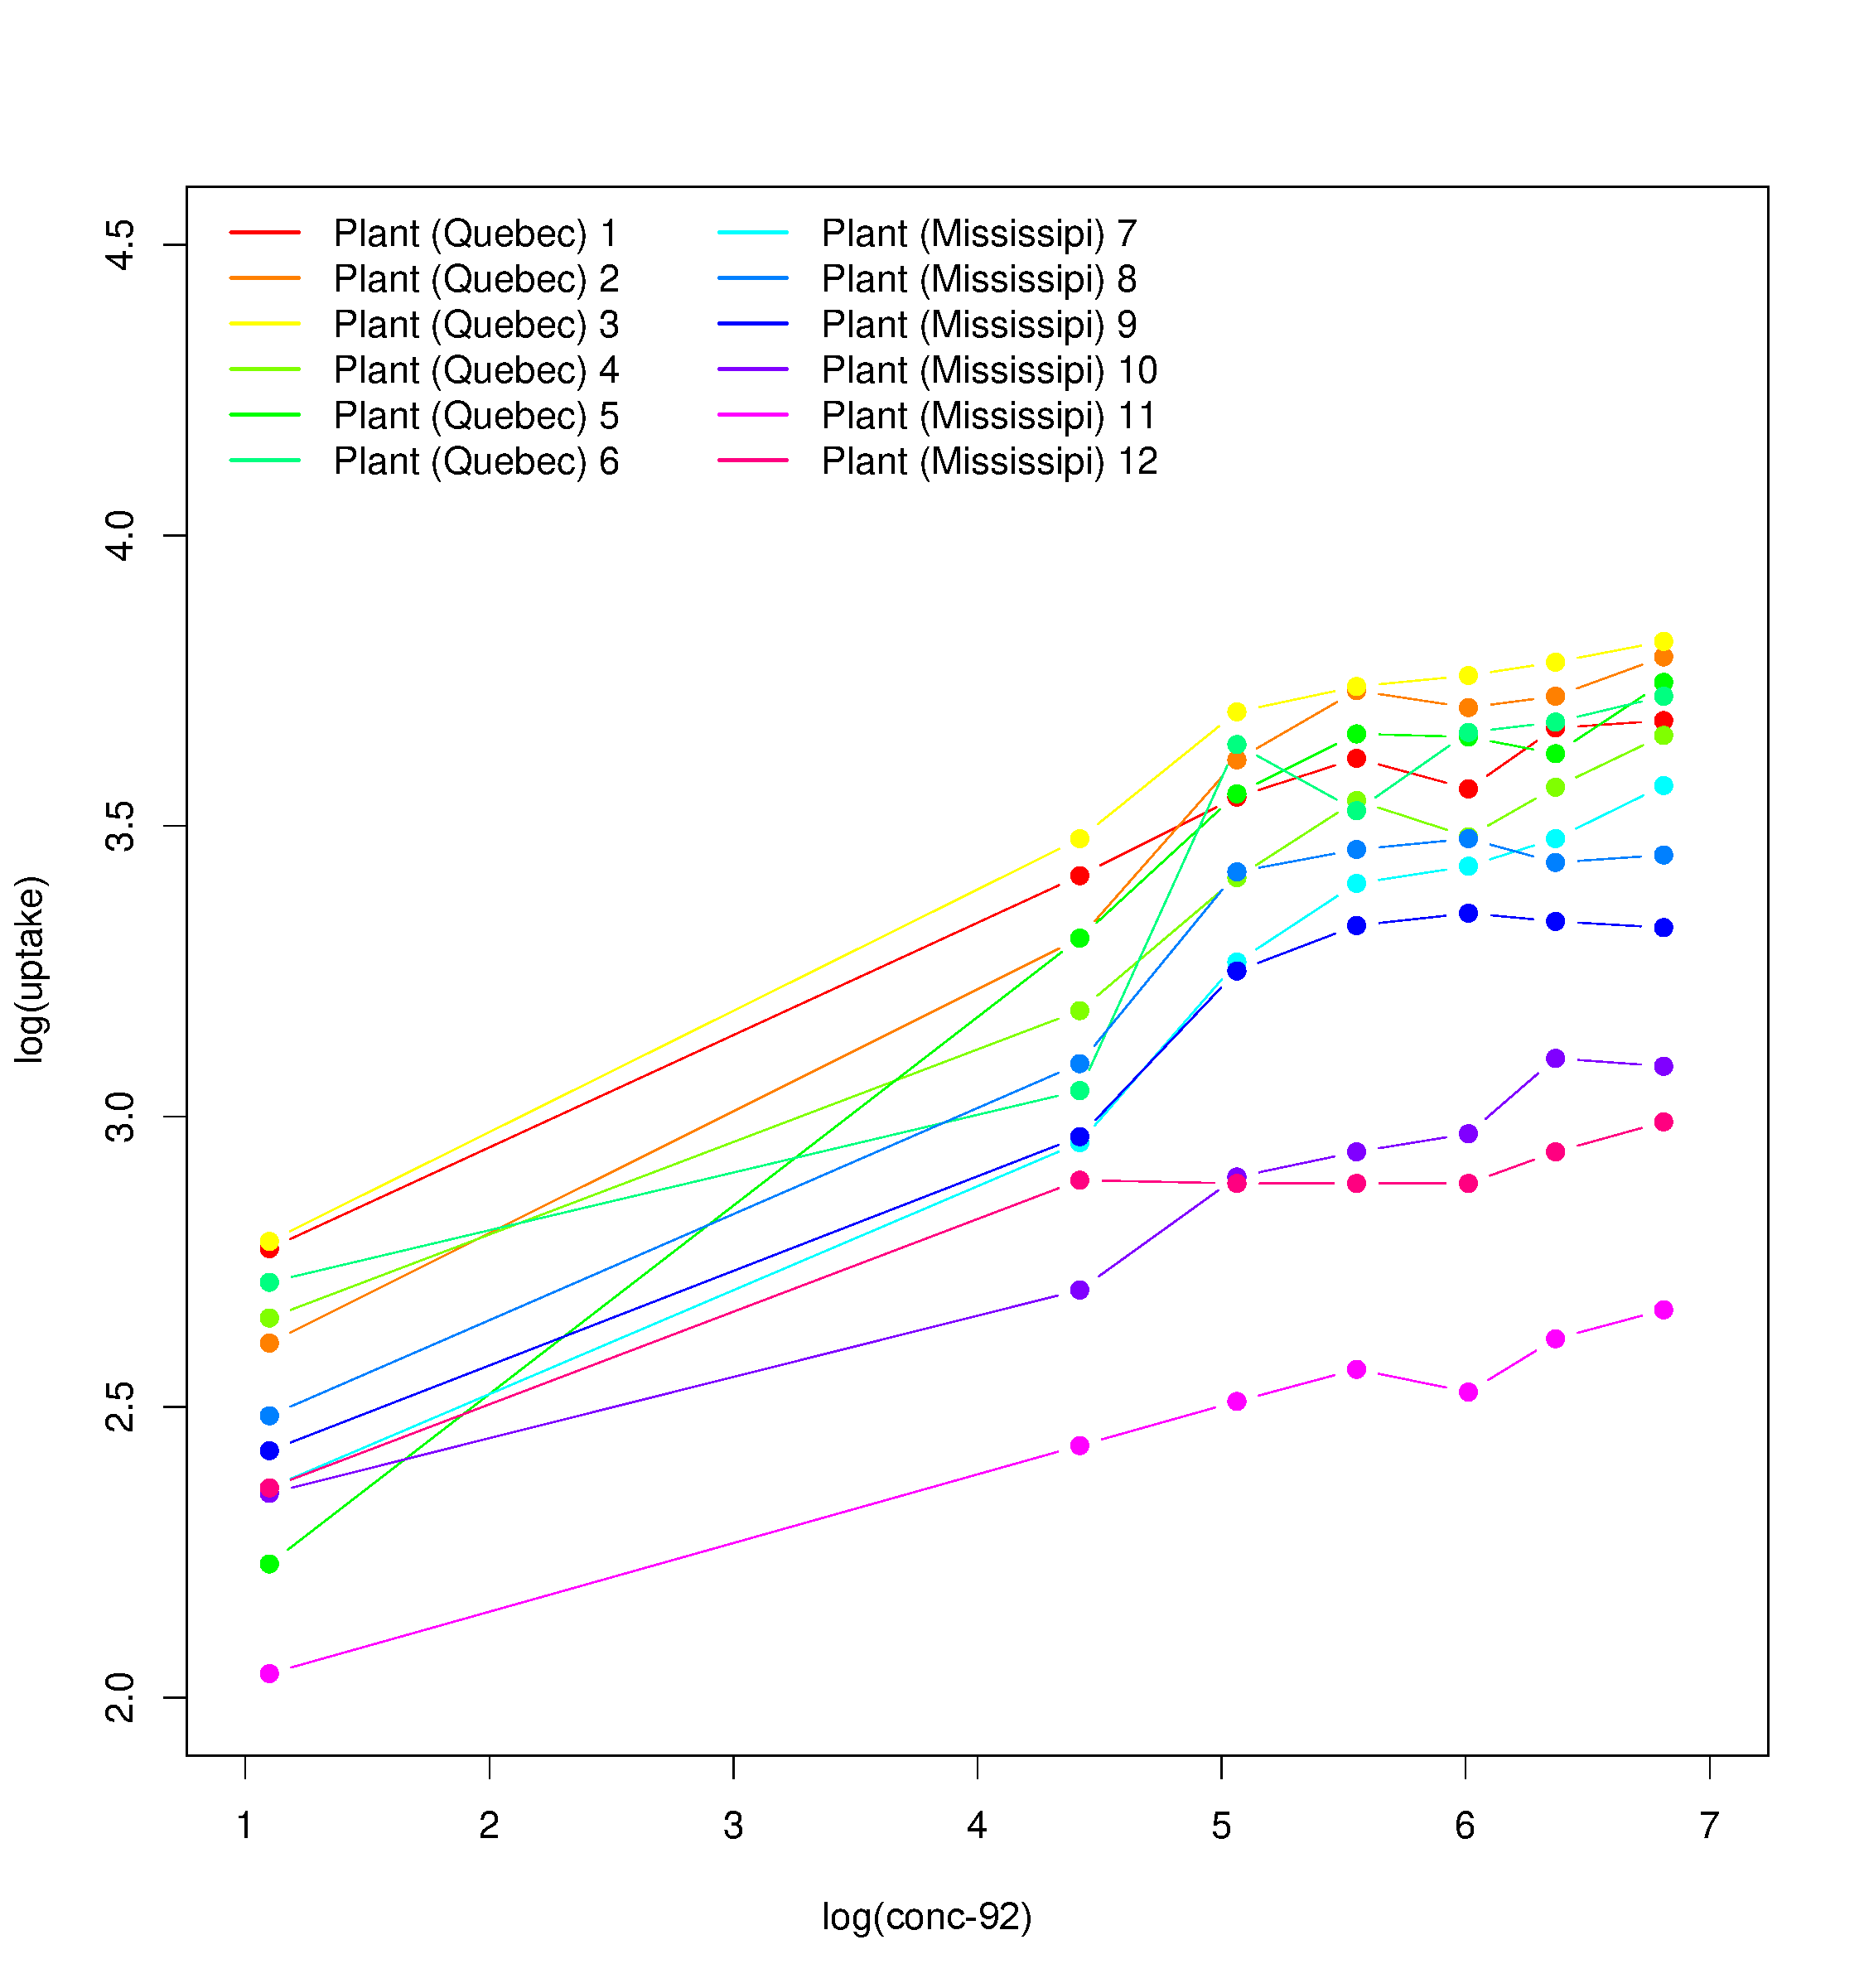
\includegraphics[height = 6in]{fig2_exa.pdf}
		\caption{$\log(\texttt{uptake})$ versus $\log(\texttt{conc}-92)$ of CO2 for each of the 12 plants.}
		\label{fig:fig_3}
	\end{figure}
	

\question[2]  Is it reasonable to assume that observations coming from a same plant are idenpendent as in the GLM models? If not, give two ways to adress this issue.
\begin{solution}
	No. It is clear from Figure \ref{fig:fig_3} that observations coming from a same plant are not independent. We could address this issue by fitting a GEE or a GLMM. 
\end{solution}
\question[3] We fitted a GLMM model to the CO2 data, see Output~\ref{out.glmm}. Write the model with precise mathematical notation. Explain what is random and what is not and state the assumptions on the random quantities.
\begin{solution}
	If $i$ indexes plants, and $k$ indexes measurements, the model is as follow : 
	$$\log(\texttt{uptake})_{ik} = \alpha + \beta_1 \log(\texttt{conc}-92)_{ik} + \beta_2 \texttt{Treatment}_{ik} +  \beta_3 \texttt{Type}_{ik} + \gamma_i + \varepsilon_{ik}$$ 
	where $\alpha$, $\beta_1$, $\beta_2$ and $\beta_3$ are non-random. $\gamma_i$ and $\varepsilon_{ik}$  are random with $\gamma_i \sim {\mathcal N}(0,\sigma^2_{\gamma})$, $\varepsilon_{ik} \sim {\mathcal N}(0,\sigma^2_{e})$ with $\gamma_j$ and $ \varepsilon_{ik}$ independent for all $i,j, k$. In fact,  \texttt{Treatment} and \texttt{Type} are time independent and therefore $\texttt{Treatment}_{ik} = \texttt{Treatment}_{i}$ and $\texttt{Type}_{ik} = \texttt{Type}_{i}$ for all $k$.
\end{solution}

\newpage
\begin{center}
\begin{verbatim}
> fit_glmm <- lmer(log(uptake) ~ log(conc-92) + Treatment + Type + (1 | Plant),  data=CO2)

> summary(fit_glmm)
Linear mixed model fit by REML ['lmerMod']
Formula: log(uptake) ~ log(conc - 92) + Treatment + Type + (1 | Plant)
   Data: CO2

REML criterion at convergence: -73.3

Scaled residuals: 
    Min      1Q  Median      3Q     Max 
-3.7805 -0.4962  0.0053  0.5037  1.9031 

Random effects:
 Groups   Name        Variance Std.Dev.
 Plant    (Intercept) 0.02043  0.1429  
 Residual             0.01466  0.1211  
Number of obs: 84, groups:  Plant, 12

Fixed effects:
                  Estimate Std. Error t value
(Intercept)       2.708464   0.083917  32.276
log(conc - 92)    0.177382   0.007446  23.823
Treatmentchilled -0.299299   0.086643  -3.454
TypeMississippi  -0.489577   0.086643  -5.650

Correlation of Fixed Effects:
            (Intr) l(-92) Trtmnt
log(cnc-92) -0.448              
Trtmntchlld -0.516  0.000       
TypeMsssspp -0.516  0.000  0.000

> logLik(fit_glmm)
'log Lik.' 36.66494 (df=6)

\end{verbatim}
\end{center}

\question[1] What is the name of the term \texttt{(1 | Plant)} in the GLMM model?

\begin{solution}
Random intercept.
\end{solution}

\question[2] Is this GLMM model performing better than Model 2 (Output~\ref{out.glm2})? Justify. 
\begin{solution}
	In addition to make more sense with the given data, this model has a way lower AIC ($-2*36.66494 + 2*6 = -61.33$) than Model 2 (AIC = -48.22): it is a better fit.
\end{solution}
\question[2] The variable \texttt{Treatment} is a 2-level factor. Only one coefficient is estimated. Explain why. 
\begin{solution}
	One of the two levels of \texttt{Treatment} is a reference level and doesn't need a coefficient since the effect of that level is already taken into account by the intercept. 
\end{solution}
\question[2] Is the effect of the variable \texttt{Treatment} significant at the $5\%$ level ? 
\label{trt.question}
\begin{solution}
The t-value associated with the \texttt{Treatment} coefficient is -3.454. The $2.5\%$ quantile of a normal distribution is $-1.96$. The variable \texttt{Treatment} is therefore significant at the $5\%$ level.
\end{solution}

\question[2] Comment on and interpret the sign of the coefficient for \texttt{Treatment}.

\begin{solution}
The sign of the coefficient of \texttt{Treatment} is negative for the level \texttt{chilled}. It indicates that chilling a plant tends to diminish it's CO2 uptake, which is expected since cold slows down plant growth. 
\end{solution}
\question[2] Based on the Output~\ref{out.glmm} and given the predictions of the random effects in Output~\ref{out.glmm.ref},  predict the \underline{value of uptake} for the Plant \texttt{Qn3}, from Quebec, for which $\log(\texttt{conc}-92) = 3$ under a chilled treatment. 

\newpage
\begin{center}
\begin{verbatim}
> ranef(fit_glmm)
$Plant
     (Intercept)
Qn1 -0.12415774
Qn2 -0.09634598
Qn3 -0.02163654
Qc1  0.04720421
Qc3  0.11129942
Qc2  0.08363664
Mn3  0.02355423
Mn2  0.13265581
Mn1  0.08593023
Mc2 -0.30362231
Mc3  0.01718117
Mc1  0.04430088
\end{verbatim}
\end{center}



\begin{solution}
Using Output \ref{out.glmm} and \ref{out.glmm.ref}: 
$\log(\texttt{uptake}) = 2.71 + 0.177 \times 3 - 0.299 + 0 - 0.022 = 2.92$
and therefore $\texttt{uptake} = \exp(2.92) = 18.54$.
\end{solution}

\question[2] For some types of GLMMs a numerical procedure is required.  Explain in which cases and why it is needed. Name two such numerical approximation procedures.
\begin{solution}
Except for the Gaussian family, the marginal likelihood is an integral that cannot be solved analytically. The numerical options to solve it include Laplace approximation, (adaptive) Gaussian quadrature, Monte Carlo approximation.
\end{solution}

 \fullwidth{We fitted a GAMM (generalized additive mixed model) with a random intercept to account for possible non linearity in the relationship between $\log(\texttt{uptake})$ and $\log(\texttt{conc}-92)$, see Output \ref{out.gamm} and Figure~\ref{fig:fig_gamm}. }
 


\begin{center}
\begin{verbatim}	
> fit_gamm <- gamm4(log(uptake) ~ s(log(conc-92), k = 7) + Treatment + Type + (1|Plant), 
   data = CO2) 
   
> summary(fit_gamm)
Family: gaussian 
Link function: identity 

Formula:
log(uptake) ~ s(log(conc-92), k = 7) + Treatment + Type + (1|Plant)

Linear mixed model fit by REML ['lmerMod']
REML criterion at convergence: -81.6

Scaled residuals: 
Min      1Q  Median      3Q     Max 
-3.9470 -0.4795  0.0591  0.4419  2.4111 

Random effects:
Groups   Name        Variance Std.Dev.
Plant    (Intercept) 0.02081  0.1443  
Residual             0.01196  0.1094  
Number of obs: 84, groups:  Plant, 12; Xr, 5

Fixed effects:
Estimate Std. Error t value
X(Intercept)       3.60358    0.07504  48.025
XTreatmentchilled -0.29930    0.08664  -3.454
XTypeMississippi  -0.48958    0.08664  -5.650
Xs(log(conc-92))Fx1     0.19013    0.07723   2.462

Correlation of Fixed Effects:
X(Int) XTrtmn XTypMs
XTrtmntchll -0.577              
XTypMsssspp -0.577  0.000       
Xs(lgcnc)F1  0.000  0.000  0.000

AIC:  -67.6035

Approximate significance of smooth terms:
           edf    Ref.df  F      p-value    
s(log(conc-92)) 3.524  3.524   202.3  <2e-16 ***

Estimated degrees of freedom: 3.52  total = 6.52 
R-sq.(adj) =  0.864   
lmer.REML = -81.603  Scale est. = 0.01196   n = 84

> gam.check(fit_gamm)
Basis dimension (k) checking results. Low p-value (k-index<1) may
indicate that k is too low, especially if edf is close to k'.

           k'   edf     k-index  p-value    
s(log(conc-92)) 6.00 3.52    0.39     <2e-16 ***
---

\end{verbatim}
\end{center}

\begin{figure}[htbp]
	\begin{center}
		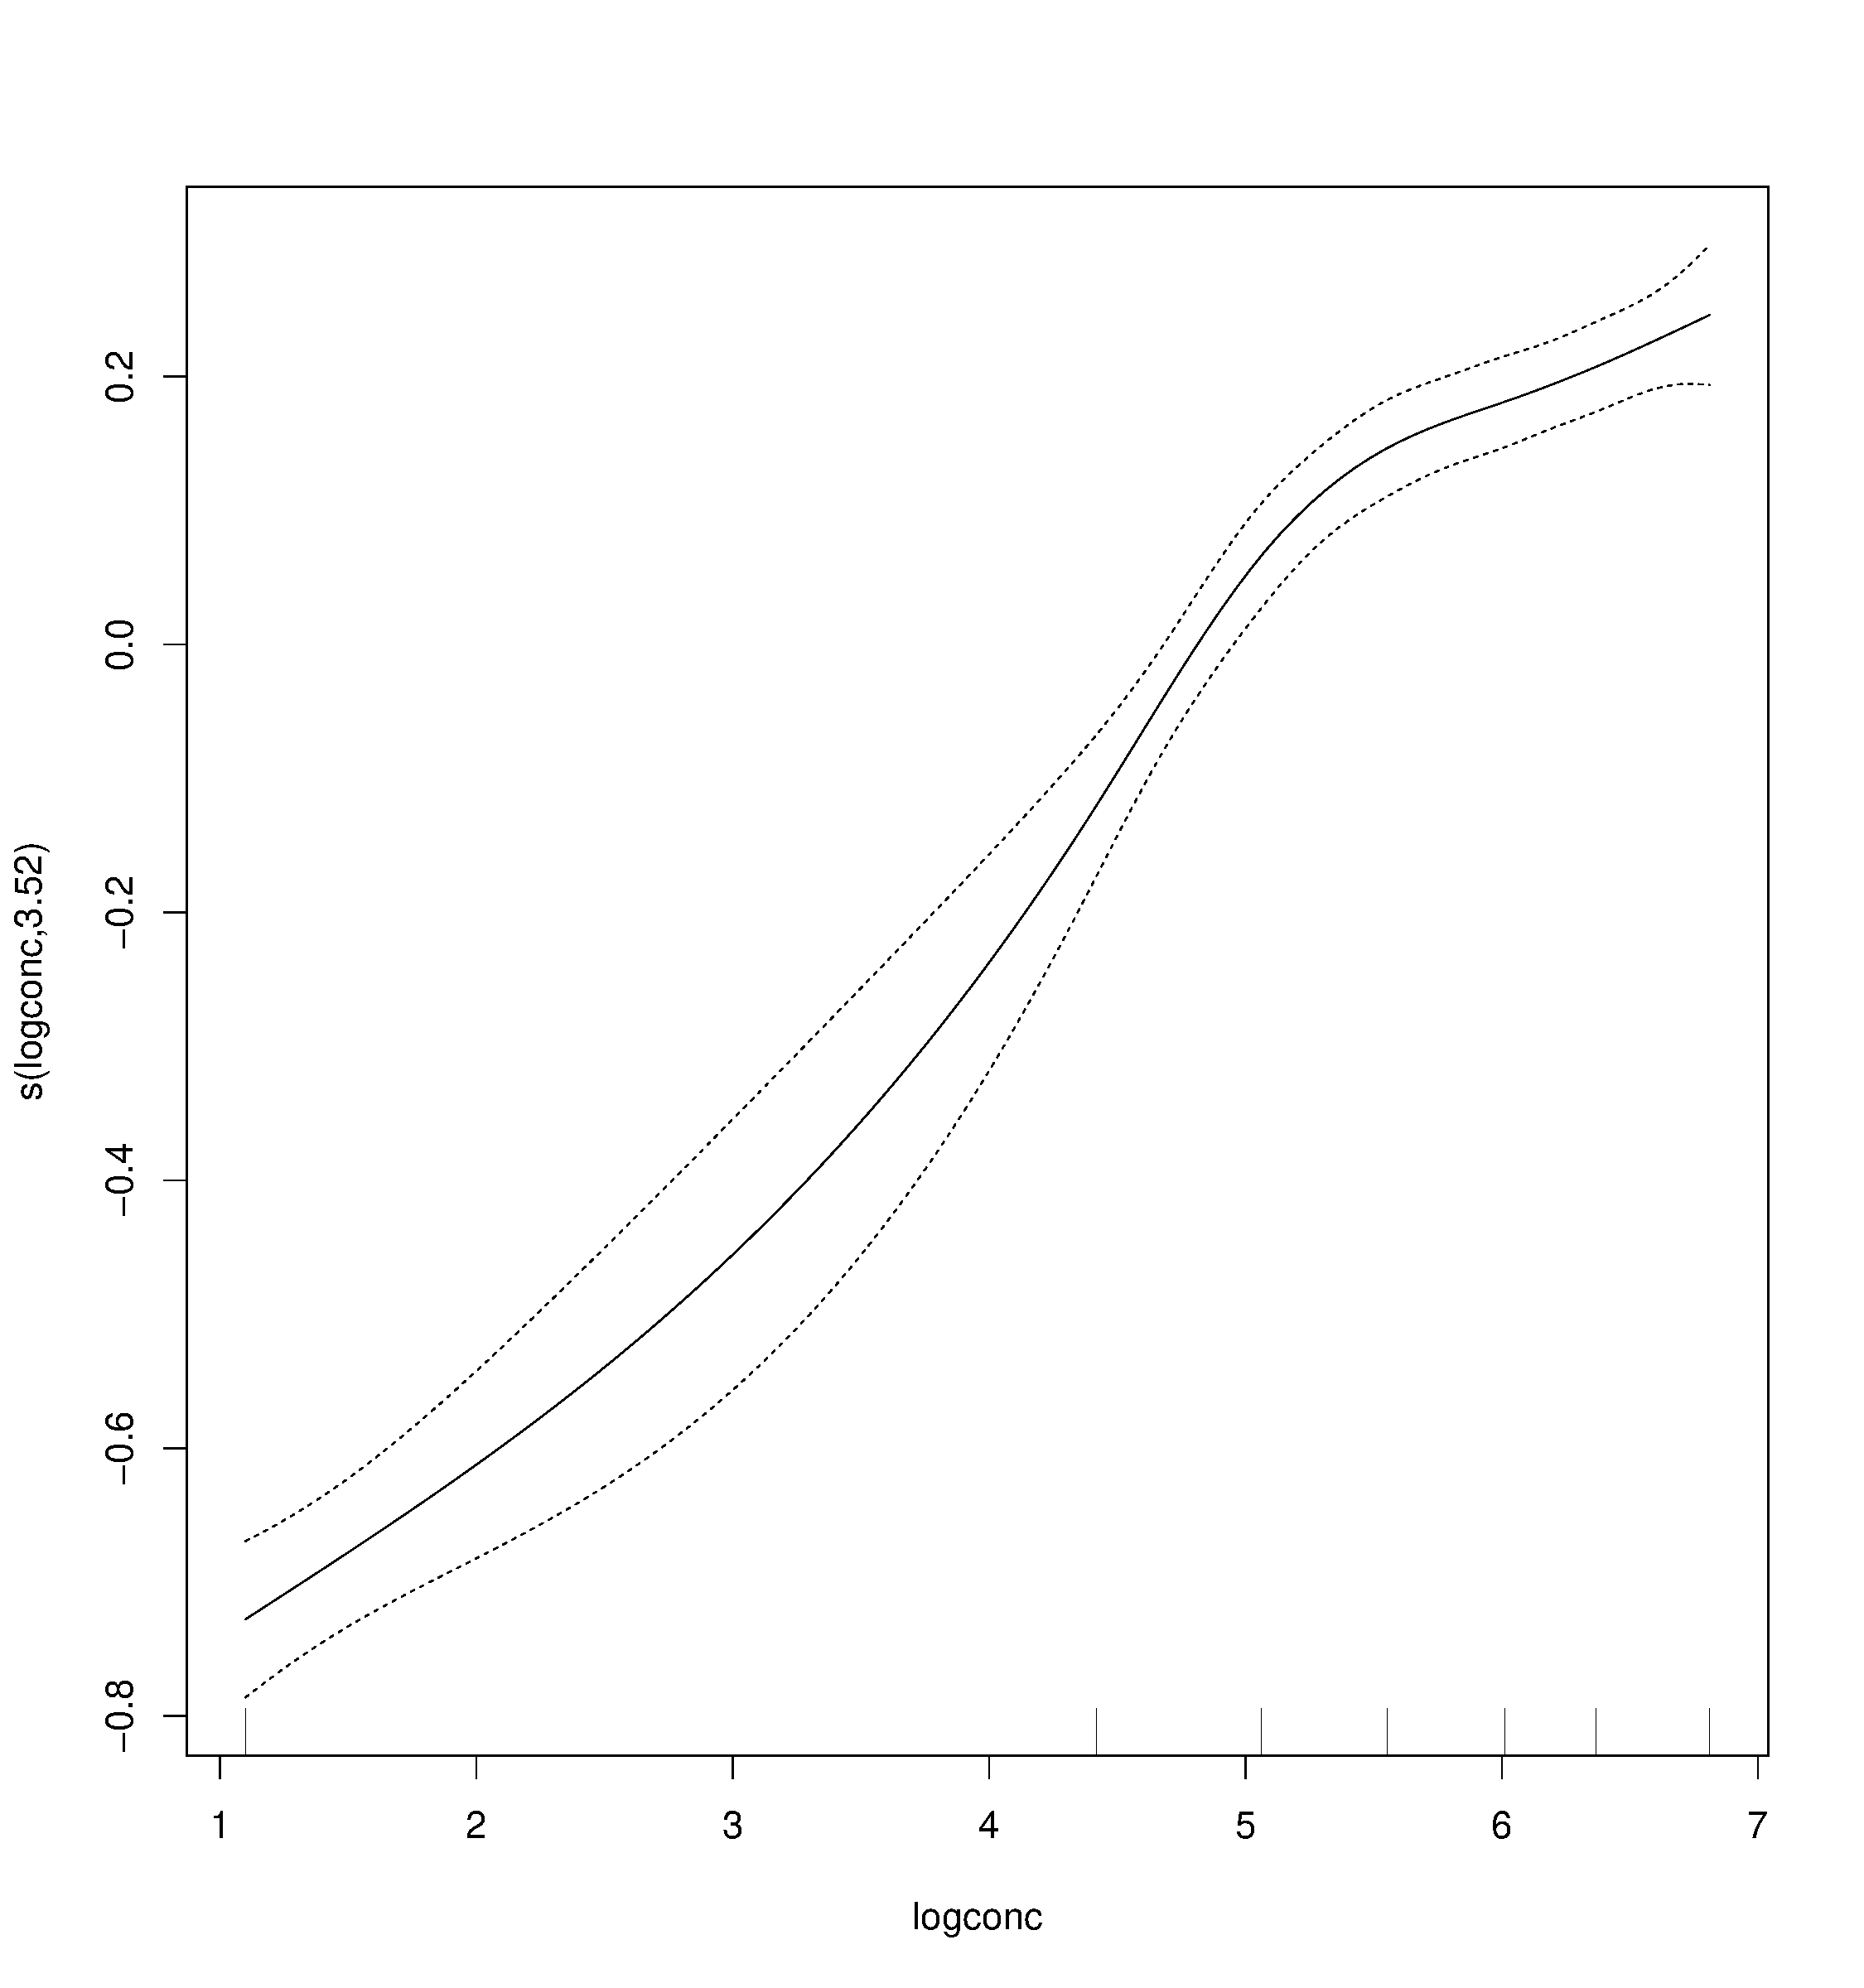
\includegraphics[height = 3in]{fig_gamm_exa.pdf}
		\label{fig:fig_4}
	\end{center}
	\caption{Fitted \texttt{s(log(conc-92))} term in the GAMM model.}
			\label{fig:fig_gamm}
\end{figure}

\question[1] Can we compare the AIC of the GAMM model with the AIC of the GLMM model ? Explain. 

\begin{solution}
Yes, the AICs can be compared: the GLMM model of Output~\ref{out.glmm} is nested in the GAMM model of Output~\ref{out.gamm}. (a linear fit is nested in a spline fit)
\end{solution}

\question[1]  Does the GAMM model improve over the GLMM Model ? Justify your answer.

\begin{solution}
Yes, the AIC of the GAMM model is -67.60, lower than the AIC of the GLMM model (-61.33).
\end{solution}

\question[1] Does your conclusion given at point \ref{trt.question}. change with the GAMM model ?

\begin{solution}
No, the estimated coefficient for \texttt{Treatment} is almost the same and the conclusions do not change.
\end{solution}

\question[2] Is the number of basis functions associated to $\log(\texttt{conc}-92)$ enough, based on Output~\ref{out.gamm}? Any fit with 8 basis functions or more returns an error. Why is that ?

\begin{solution}
\texttt{gam.check()} seems to indicate that 7 basis functions are not enough, but their number cannot be increased because we see from Figure~\ref{fig:fig_3} that the variable $\log(\texttt{conc}-92)$ only takes 7 distinct values.
\end{solution}



\question[2]  Is the smooth term on  $\log(\texttt{conc}-92)$  worth with respect to a linear fit? Justify your answer.

\begin{solution}
Yes, the smooth term is worth. The approximate significance of smooth terms test is significant, therefore there is evidence of non linearity. 

Other justifications:\\
- AIC of the GAMM model improved over GLMM model (only difference is the  $\log(\texttt{conc}-92)$  term.\\
- a straight line cannot be fitted within the confidence bands.
\end{solution}


\question[1] Would adding a spline on the variable \texttt{Treatment} be relevant ?
\begin{solution}
No, because  \texttt{Treatment} is a dummy variable. Smooth terms are only for continuous variables.
\end{solution}


\end{questions}

\newpage
{\Large \textbf{Exercise 2} \hfill (18 points)}

For the \underline{Gaussian family with identity link} (like in the previous exercise), we would like to show that the maximum likelihood estimator of the regression parameter $\beta$ in a random intercept GLMM is equivalent to the estimator of $\beta$ in the GEE approach with exchangeable correlation matrix, \textbf{when the variance/nuisance parameters are known}.

Let $Y_{it}$ denote the response of individual $i$ at time $t$, for $i=1,\ldots,n$ and $t=1,\ldots,n_i$. We assume a normal distribution for
$Y_{it}$ and we define a linear predictor $x_{it}^T\beta$, where both $x_{it}$ and $\beta$ are of dimension $(p+1) \times 1$ and $x_{it}$ is non-random.

\bigskip

We first consider a random intercept GLMM specification as follows
\begin{equation}\label{glmm.model}
    Y_{it}=x_{it}^T\beta+\gamma_i+\epsilon_{it},
\end{equation}
where we assume $\gamma_i\overset{\text{i.i.d.}}{\sim}N(0,\sigma^2_\gamma)$, $\epsilon_{it}\overset{\text{i.i.d.}}{\sim} N(0,\sigma^2_\epsilon)$, with $\gamma_i$  and $\epsilon_{jt}$ independent $\forall i, j, t$. We assume that $\sigma^2_\gamma$ and $\sigma^2_\epsilon$ are known.

Model~\eqref{glmm.model} can equivalently be written as
\begin{equation}\label{glmm.model.vector}
    Y_i=X_i\beta+u_i,
\end{equation}
where $Y_i = (Y_{i1},\ldots,Y_{in_i})^T$, $X_i = (x_{i1}, \cdots, x_{in_i})^T$ and $u_i=(u_{i1},\ldots,u_{in_i})^T$, with $u_i \sim N(0,\Omega_i)$.\\


\textit{Reminder}: If $Z = (Z_1,\ldots,Z_k)\sim N(\mu,\Sigma)$, its density is $$f(z) = (2\pi)^{-k/2} |\Sigma|^{-1/2}
\exp\left(-\frac{1}{2}\left(z-\mu \right)^T\Sigma^{-1}\left(z-\mu\right) \right),$$
where $|\Sigma|$ denotes the determinant of $\Sigma$.

\begin{questions}
\question[3] Show that $Cov[Y_{it},Y_{is}]$ equals $\sigma^2_\gamma+\sigma^2_\epsilon$ if $t=s$, and equals $\sigma^2_\gamma$ if $t\neq s$.
\begin{solution}
$$
\begin{array}{ccl}
Cov(Y_{it}, Y_{is}) & = & Cov(x_{it}\beta + \gamma_i + \epsilon_{it}, x_{is}\beta + \gamma_i + \epsilon_{is})\\
 & = & Cov(\gamma_i + \epsilon_{it}, \gamma_i + \epsilon_{is})\\
 & = & Cov(\gamma_i, \gamma_i) + Cov(\gamma_i, \epsilon_{is}) + Cov(\epsilon_{it}, \gamma_i) + Cov(\epsilon_{it}, \epsilon_{is})\\
 & = & \textrm{var}(\gamma_i) + 0 + 0 + Cov(\epsilon_{it}, \epsilon_{is})
 \end{array}
 $$
 As $\epsilon_{is}$ and $\epsilon_{it}$ are independent if $t\neq s$, $Cov(\epsilon_{it}, \epsilon_{is}) = \left\{\begin{array}{ccl} 0 &\,\,\textrm{if}\,\, & t \neq s\\ var(\epsilon_{it}) & \,\,\textrm{if}\,\, & t = s\end{array}\right.$
 Hence, $Cov(Y_{it}, Y_{is}) = \sigma_\gamma^2$ if $t\neq s$ and $Cov(Y_{it}, Y_{is}) = \sigma_\gamma^2 + \sigma_\epsilon^2$ if $t =s$. 

\end{solution}

\question[2] Define $u_i$ as a function of $\gamma_i$ and $\epsilon_i =
(\epsilon_{i1}, \ldots, \epsilon_{in_i})^T$. 
\begin{solution}
	$ Y_{it}=x_{it}^T\beta+\gamma_i+\epsilon_{it}$ is equivalent to, 
	$$Y = X\beta + \left(\begin{array}{c}\gamma_i\\ \vdots \\ \gamma_i\end{array}\right) + \left(\begin{array}{c}\epsilon_{i1}\\ \vdots \\ \epsilon_{i n_i}\end{array}\right) = X_i \beta + \left(\begin{array}{c}\gamma_i + \epsilon_{i1}\\ \vdots \\ \gamma_i + \epsilon_{i n_i}\end{array}\right) \, . $$ Hence $u_i = \left(\begin{array}{c}\gamma_i + \epsilon_{i1}\\ \vdots \\ \gamma_i + \epsilon_{i n_i}\end{array}\right)$.
\end{solution}
\question[2] Give $\Omega_i$ explicitly (by making clear what are its dimensions).
\begin{solution}
	$ cov({u_i}_t, {u_i}_s) = cov(\gamma_i + \epsilon_{it}, \gamma_i + \epsilon_{is}) = \left\{
	\begin{array}{ccl}\sigma_\gamma^2&\text{if}& t\neq s\\ \sigma_\gamma^2 + \sigma_\epsilon^2& \text{if} & t = s \end{array}\right.$. 
	Hence $$ \Omega_i = 
	\left(\begin{array}{cccc} 
	 \sigma_\gamma^2 + \sigma_\epsilon^2 & \sigma_\gamma^2 & \cdots & \sigma_\gamma^2\\
	 \sigma_\gamma^2 & \sigma_\gamma^2 + \sigma_\epsilon^2 & \ddots& \vdots \\
	 \vdots & \ddots& \ddots & 	\sigma_\gamma^2 \\
	 \sigma_\gamma^2  & \cdots & \sigma_\gamma^2 & \sigma_\gamma^2 + \sigma_\epsilon^2
	\end{array}\right).$$ This matrix is of dimension $n_i \times n_i$. 
\end{solution}
\question[2] What is the distribution of $Y_i$?
\begin{solution}
	As $u_i \sim \mathcal{N}(0, \Omega_i)$ and $Y_i = X_i \beta +u_i$, $Y_i \sim \mathcal{N}(X_i \beta, \Omega_i)$.
\end{solution}
\question[3] \label{glmm}Assuming $\Omega_i$ known $\forall i$, compute the likelihood function
$L(\beta | Y_1, \ldots, Y_n, \Omega_1, \ldots,\Omega_n)$
and give the estimating (score) equations for the maximum likelihood estimator
of $\beta$.
\begin{solution}
	$$\begin{array}{ccl}
	L(\beta\mid Y_1, \cdots, Y_n, \Omega_1, \cdots , \Omega_n) & = & \prod_{i = 1}^{n} \frac{(2\pi)^{n_i / 2}}{\lvert \Omega_i\rvert^{1/2}} \exp\left((Y_i - X_i\beta)^T \Omega_i^{-1}(Y_i - X_i\beta)
	 \right))\\
	 l(\beta\mid Y_1, \cdots, Y_n, \Omega_1, \cdots , \Omega_n) & = & \sum_{i = 1}^{n} \log(\frac{(2\pi)^{n_i / 2}}{\lvert \Omega_i\rvert^{1/2}}) + (Y_i - X_i\beta)^T \Omega_i^{-1}(Y_i - X_i\beta)\\
	 \frac{\partial l}{\partial \beta}(\beta\mid Y_1, \cdots, Y_n, \Omega_1, \cdots , \Omega_n) & = & \sum_{i = 1}^{n} 2 X_i^T  \Omega_i^{-1}(Y_i - X_i\beta)\\
	 \end{array} .$$
	 
	 Hence the estimating equation of the GLMM is 
	 $$\sum_{i = 1}^{n} X_i^T \Omega_i^{-1}(Y_i - X_i\beta) = 0. $$  
\end{solution}

\bigskip

\fullwidth{We next consider a GEE specification with exchangeable correlation, that is
\begin{equation*}
E[Y_{it}]=\mu_{it}=x_{it}^T\beta,
\end{equation*}
where we set $Var[Y_{it}]=\tau^2$ and the working correlation matrix $R_i(\alpha)$ such that its $(t,s)$ element is equal to $\alpha$, for $t \neq s$ and to 1 otherwise. We assume that $\tau^2$ and $\alpha$ are known.}

\question[3] \label{gee}Write explicitly the model estimating equations under this setting, based on the lecture slides (p.~190) and give the working covariance matrix $V_i = V_i(\alpha,\tau^2)$ explicitely.
\begin{solution}
	Lecture slide 190 give that the estimating equation is : 
$$\sum_{i = 1}^{n} \left(\frac{\partial \mu_i}{\partial \beta}\right)^TV_i^{-1}(Y_i -  \mu_i) = 0,$$
where $V_i = A_i^{1/2} R_i(\alpha)A_i^{1/2}$ whith $A_i$ a diagonal matrix with variances of $Y_{i1},  \cdots, Y_{in_i}$ on its diagonal elements. 
Here, for any $t\in\{1,\cdots n_i\}$, $var(Y_{it}) = \tau^2$ such that
$V_i = \tau^2 R_i(\alpha)$. Besides, $\mu_i = X_i \beta$ and $\frac{\partial \mu_i}{\partial \beta} = X_i$. Hence the estimating equation rewrites
$$\sum_{i = 1}^{n} X_i^T \tau^{-2} R_i(\alpha)^{-1}(Y_i -  \mu_i) = 0.$$ 
\end{solution}
\question[2] Compare the estimating equations found in \ref{glmm}. and \ref{gee}. What do you conclude for these two specifications under this specific setting?
What is the relationship between $\sigma^2_\gamma$, $\sigma^2_\epsilon$, $\tau^2$ and $\alpha$? And between $R_i(\alpha)$ and $\Omega_i$?
\begin{solution}
Notice that the matrices $\Omega_i$ and $\tau^2 R_i(\alpha)$ have the same structure. 
Indeed, if 
$$\left\{\begin{array}{ccc}
	\tau^2 & = &\sigma_\epsilon^2 + \sigma_\gamma^2\\
	\alpha \tau^2 & = &\sigma_\gamma^2
\end{array}\right. \Longleftrightarrow \left\{\begin{array}{ccc}
\tau^2 & = &\sigma_\epsilon^2 + \sigma_\gamma^2\\
\alpha & = &\frac{\sigma_\gamma^2}{\sigma_\epsilon^2 + \sigma_\gamma^2}
\end{array}\right. \, ,$$
$\Omega_i = \tau^2 V_i$ for all $i \in \{1,\cdots n\}$ and the estimating equations for $\beta$ of the GEE and GLMM models become indentical. 

\end{solution}

\begin{center}
	\begin{verbatim}
> fit_gee <- gee(log(uptake) ~ log(conc-92) + Treatment + Type, id = Plant, 
  corstr = "exchangeable")	

> summary(fit_gee)
 GEE:  GENERALIZED LINEAR MODELS FOR DEPENDENT DATA
gee S-function, version 4.13 modified 98/01/27 (1998) 

Model:
Link:                      Identity 
Variance to Mean Relation: Gaussian 
Correlation Structure:     Exchangeable 

Call:
gee(formula = log(uptake) ~ log(conc-92) + Treatment + Type, id = Plant, 
corstr = "exchangeable")

Summary of Residuals:
Min          1Q      Median          3Q         Max 
-0.46055369 -0.09947886  0.01697381  0.12597427  0.33303499 


Coefficients:
Estimate  Naive S.E.   Naive z Robust S.E.  Robust z
(Intercept)       2.7084641 0.076396145 35.452890  0.09097667 29.770975
log(conc-92)      0.1773822 0.007700858 23.034085  0.01300256 13.642101
Treatmentchilled -0.2992991 0.075949456 -3.940767  0.07503523 -3.988780
TypeMississippi  -0.4895767 0.075949456 -6.446085  0.07503523 -6.524624

Estimated Scale Parameter:  0.0307418
Number of Iterations:  1

Working Correlation
[,1]      [,2]      [,3]      [,4]      [,5]      [,6]      [,7]
[1,] 1.0000000 0.4900651 0.4900651 0.4900651 0.4900651 0.4900651 0.4900651
[2,] 0.4900651 1.0000000 0.4900651 0.4900651 0.4900651 0.4900651 0.4900651
[3,] 0.4900651 0.4900651 1.0000000 0.4900651 0.4900651 0.4900651 0.4900651
[4,] 0.4900651 0.4900651 0.4900651 1.0000000 0.4900651 0.4900651 0.4900651
[5,] 0.4900651 0.4900651 0.4900651 0.4900651 1.0000000 0.4900651 0.4900651
[6,] 0.4900651 0.4900651 0.4900651 0.4900651 0.4900651 1.0000000 0.4900651
[7,] 0.4900651 0.4900651 0.4900651 0.4900651 0.4900651 0.4900651 1.0000000
	\end{verbatim}
\end{center}

\question[1] We fitted a GEE model on the CO2 data. Output \ref{out.gee} shows a summary of this fit. Compare it to the GLMM Model summarized in Output \ref{out.glmm} of the previous exercise. What do you notice ? Comment. 

\begin{solution}
We observe that the regression parameter estimates ($\hat{\beta}$) are the same on both models, as expected. And this, even though the nuisance parameters are estimated.
\end{solution}

\end{questions}



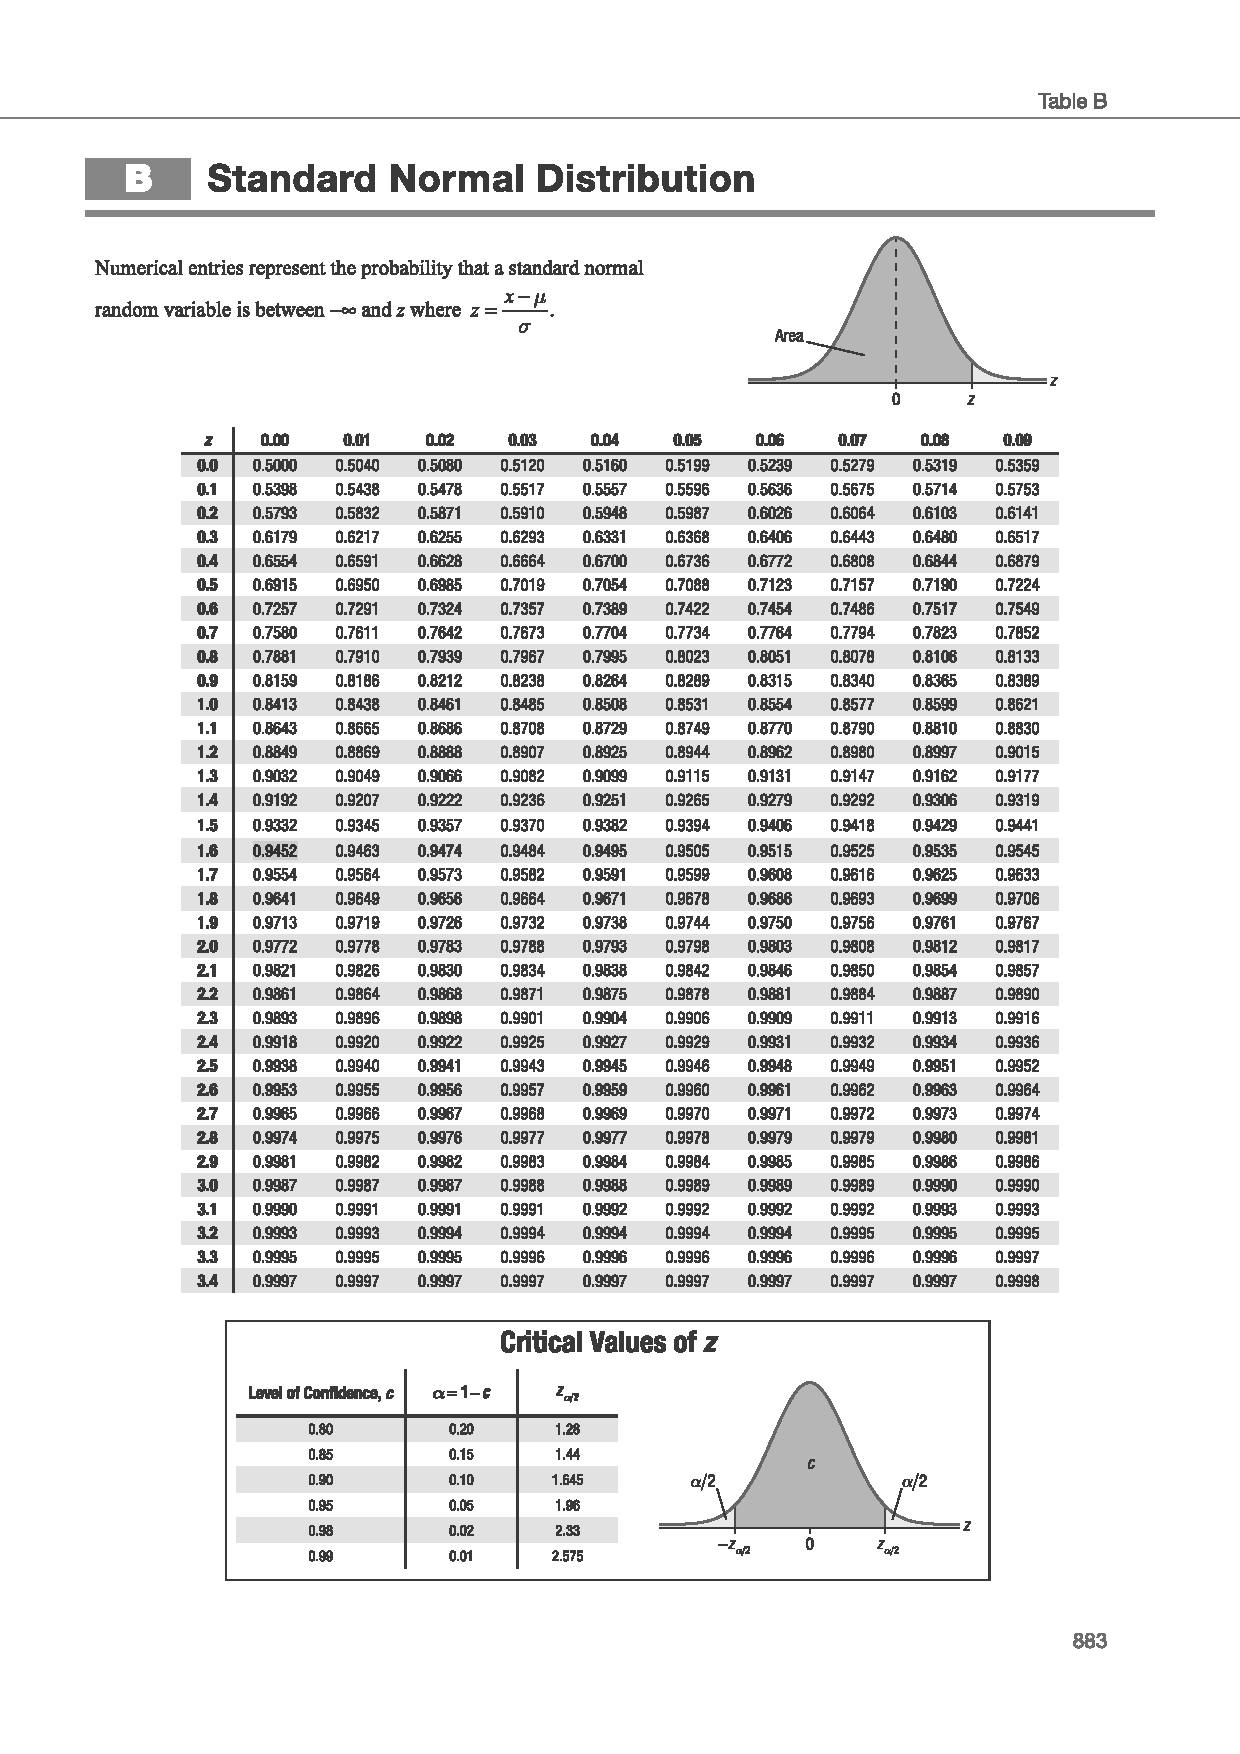
\includepdf[pages=-]{tables_norm_chisq.pdf}

\end{document}

